\chapter{البلاستيك والمواد الاصطناعية}\label{ch:g8:plastics}

عُدّ الأجسام البلاستيكية التي تلمسها في صباح واحد: فرشاة الأسنان، والقارورة،
ومعطف المطر، وغطاء الهاتف، ومقعد الحافلة، وكيس التسوق. لم يكن أي منها
تقريبًا موجودًا قبل مئة وعشرين سنة، ولم ينبت أي منها على شجرة ولا استُخرج
من باطن الأرض. \omterm{def:g8:plastics:plastic}{البلاستيك} مواد اخترعها الكيميائيون --- خفيفة، ورخيصة،
وكتيمة للماء، وتتشكل على أي هيئة --- وهذا النجاح نفسه صار مشكلة.

\begin{recall}
المواد الطبيعية تُستعمل كما توجد في الطبيعة تقريبًا؛ والمواد المصنّعة تُصنع
من المواد الأولية بتغييرها، \omterm{def:g5:raw-materials-and-recycling:recycling}{وإعادة التدوير} تحوّل مادة الأجسام القديمة إلى
أجسام جديدة (\cref{ch:g5:raw-materials-and-recycling}). \omterm{def:g4:what-a-fire-needs:burning}{واحتراق} \omterm{def:g4:what-a-fire-needs:fuel}{وقود}
مكوّن من الكربون والهيدروجين يعطي ثنائي أكسيد الكربون والماء
(\cref{ch:g8:combustion-and-fuels}).
\end{recall}

\begin{omfigure}
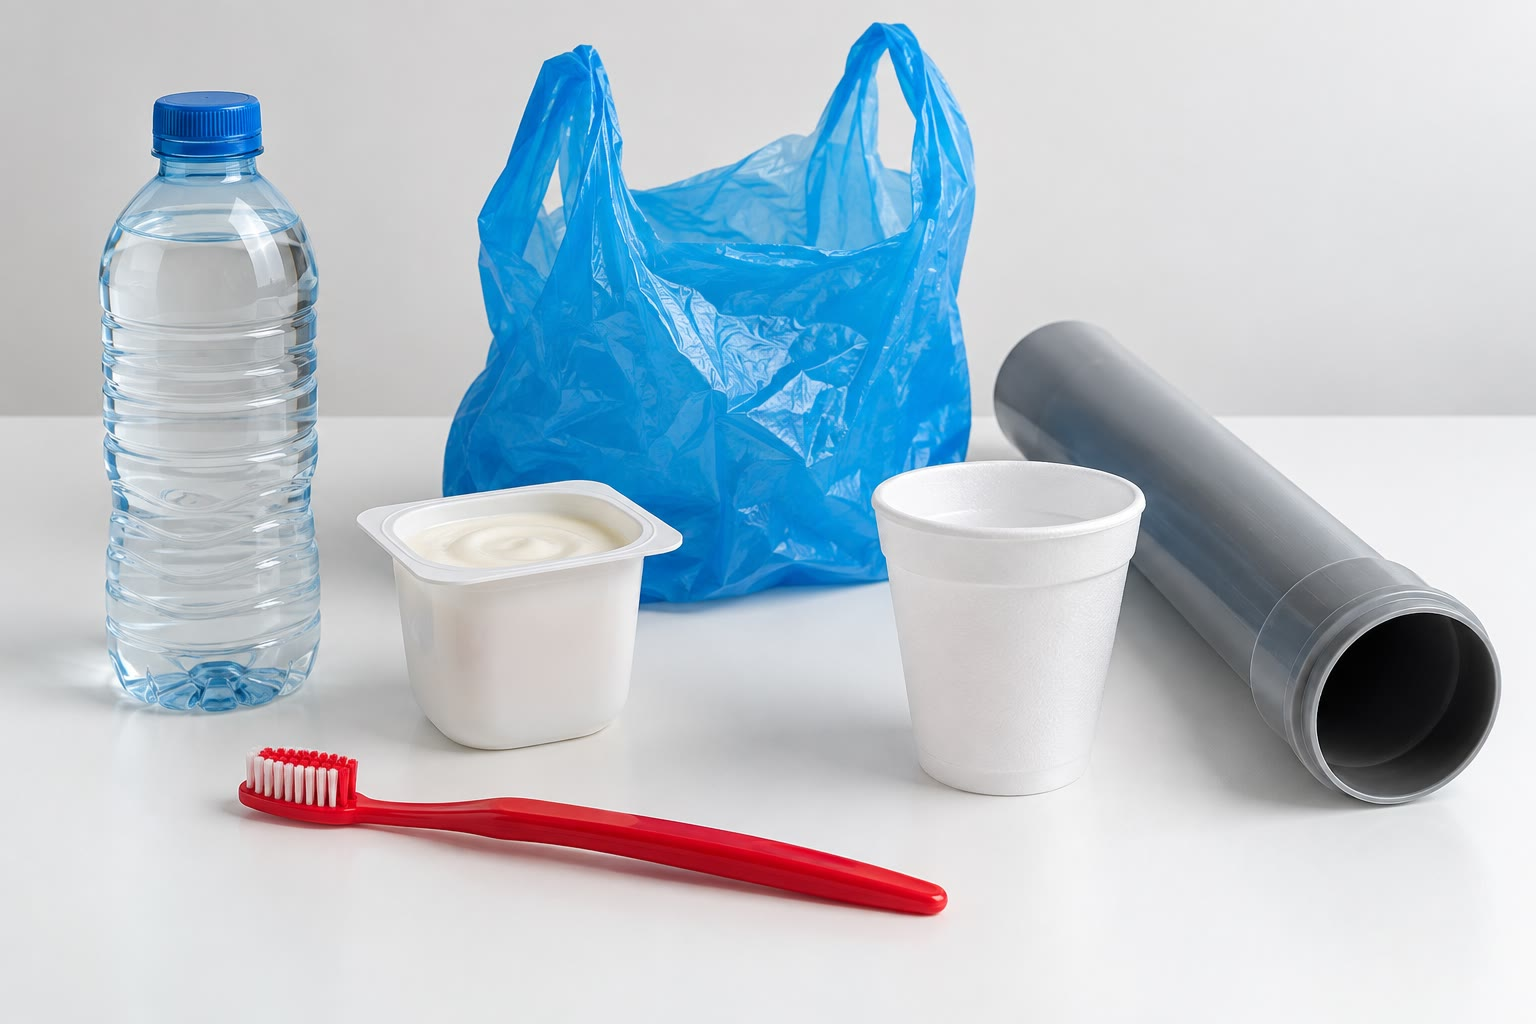
\includegraphics[width=0.55\linewidth]{images/book1/ai/g8-plastic-objects.jpg}

{\small أجسام بلاستيكية يومية: قارورة، ووعاء، وكيس، وأنبوب، وكوب، وفرشاة
أسنان.}
\end{omfigure}

\section{المواد الطبيعية والمواد الصناعية والمواد الاصطناعية}

\begin{definition}[المواد الصناعية والمواد الاصطناعية]\label{def:g8:plastics:artificial}
من بين المواد المصنّعة، تُصنع \emph{المادة الصناعية}\index{مادة صناعية}
بتحويل \omterm{def:g5:raw-materials-and-recycling:natural-material}{مادة طبيعية} تحويلًا كيميائيًا: كالورق والفسكوز (وهو نسيج) المصنوعين
من سليلوز الخشب. أما \emph{المادة الاصطناعية}\index{مادة اصطناعية} فتُصنع
من مواد بناها الكيميائيون، وفي الغالب من النفط الخام، وليس لها نظير في
الطبيعة: النايلون، والبوليستر، وأنواع \omterm{def:g8:plastics:plastic}{البلاستيك}.
\end{definition}

\begin{omfigure}
\begin{tikzpicture}[font=\small, level distance=1.5cm,
    box/.style={draw=omDef, fill=omDef!6, rounded corners=2pt, align=center,
      inner sep=4pt, text width=3.3cm},
    level 1/.style={sibling distance=6.4cm},
    level 2/.style={sibling distance=3.8cm},
    edge from parent/.style={draw, thick, omDef, ->}]
  \node[box] {المواد}
    child {node[box] {طبيعية\\ \footnotesize القطن، الصوف، الخشب}}
    child {node[box] {مصنّعة}
      child {node[box] {صناعية\\ \footnotesize الورق، الفسكوز}}
      child {node[box, draw=omProp, fill=omProp!6] {اصطناعية\\ \footnotesize النايلون،
        البوليستر، البلاستيك}}};
\end{tikzpicture}

{\small المواد الطبيعية والصناعية والاصطناعية.}
\end{omfigure}

\section{ما البلاستيك}

\begin{definition}[البلاستيك]\label{def:g8:plastics:plastic}
\emph{البلاستيك}\index{بلاستيك} \omterm{def:g8:plastics:artificial}{مادة اصطناعية} مكوّنة من \omterm{def:g7:atoms-and-molecules:molecule}{جزيئات} طويلة جدًا،
يمكن تشكيلها بالقولبة --- وفي الغالب وهي ساخنة لينة --- وتحتفظ بشكلها حين
تبرد. ومعظم أنواع البلاستيك تُصنع من النفط الخام أو الغاز الطبيعي.
\end{definition}

\begin{remark}[جزيئات طويلة جدًا]\label{rem:g8:plastics:long}
\omterm{def:g7:atoms-and-molecules:molecule}{جزيء} الماء يحوي ثلاث \omterm{def:g7:atoms-and-molecules:atom}{ذرات}؛ أما \omterm{def:g7:atoms-and-molecules:molecule}{جزيء} \omterm{def:g8:plastics:plastic}{البلاستيك} فقد يحوي عشرات الآلاف منها،
مرتبطة في سلسلة طويلة، كعقد من خرز متماثل. أما كيف تُبنى هذه السلاسل فموضوع
فصل في آخر هذا الكتاب.
\end{remark}

\begin{omfigure}
\begin{tikzpicture}[font=\small]
  \foreach \k in {0,...,17} {
    \pgfmathsetmacro\x{0.62*\k}
    \pgfmathsetmacro\y{0.35*sin(40*\k)}
    \shade[ball color=omDef!50] (\x,\y) circle (0.22);
  }
  \node[anchor=west] at (11.2,0) {\dots};
  \node[anchor=north, align=center] at (5.3,-0.6) {سلسلة من آلاف الوحدات المتماثلة};
\end{tikzpicture}

{\small صورة لا نموذج: \omterm{def:g7:atoms-and-molecules:molecule}{جزيء} \omterm{def:g8:plastics:plastic}{البلاستيك} سلسلة طويلة جدًا من وحدات
متماثلة.}
\end{omfigure}

\begin{history}[الباكليت، 1907]
صنع الكيميائي ليو بيكلاند أول \omterm{def:g8:plastics:plastic}{بلاستيك} اصطناعي بالكامل سنة 1907، من
الفينول، المستخرج من قطران الفحم، والفورمالدهيد. وصار الباكليت، الصلب
الداكن المقاوم للحرارة، مادة الهواتف وأجهزة الراديو ومفاتيح الكهرباء. ثم جاء
النايلون في ثلاثينيات القرن العشرين، ثم \omterm{def:g8:plastics:plastic}{بلاستيك} القوارير والأكياس بعد
الحرب العالمية الثانية.
\end{history}

\begin{omfigure}
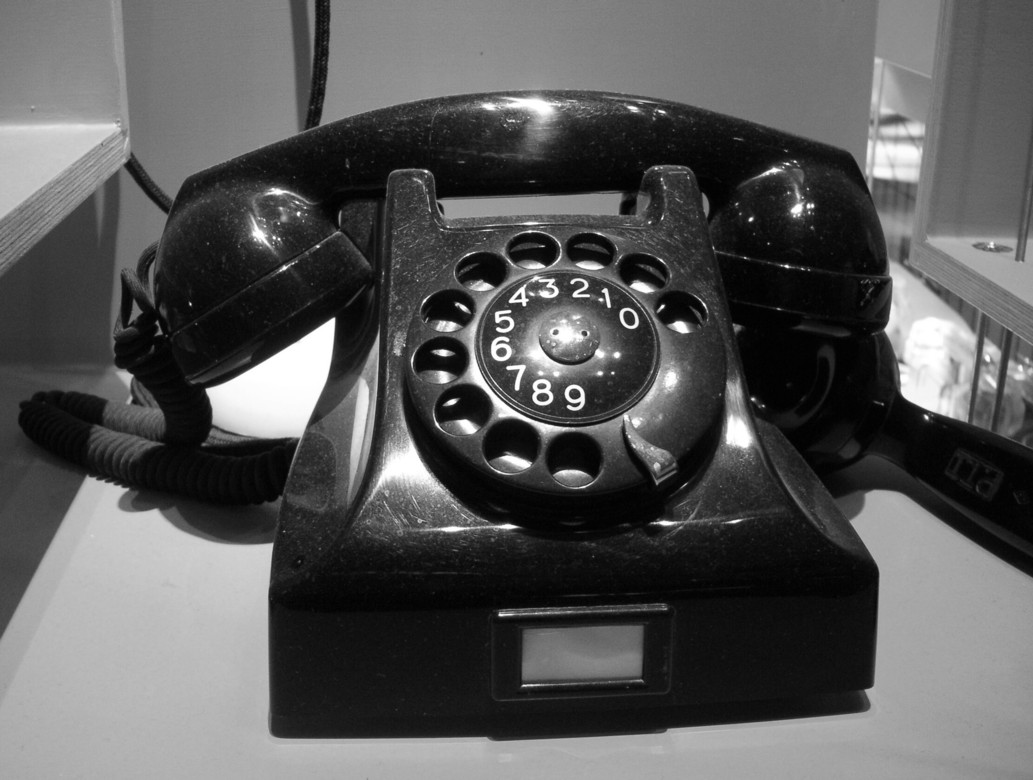
\includegraphics[width=0.42\linewidth]{images/book1/bakelite-telephone.jpg}

{\small هاتف من الباكليت من سنة 1947. تصوير: هولغر إلغارد،
CC BY-SA 3.0.}
\end{omfigure}

\section{أنواع البلاستيك الرئيسية ورموزها}

\begin{definition}[رمز تعريف الراتنج]\label{def:g8:plastics:code}
\emph{رمز تعريف الراتنج}\index{رمز تعريف الراتنج} عدد من 1 إلى 7، يُطبع
داخل مثلث من الأسهم على الجسم البلاستيكي، ويسمّي \omterm{def:g8:plastics:plastic}{البلاستيك} الذي صُنع منه،
كي يمكن فرزه \omterm{def:g5:raw-materials-and-recycling:recycling}{لإعادة التدوير}. والمثلث لا يعني أن الجسم سيُعاد
تدويره.
\end{definition}

\begin{proposition}[سبعة رموز]\label{prop:g8:plastics:codes}
الرموز، مع أشيع استعمالات كل نوع من \omterm{def:g8:plastics:plastic}{البلاستيك}:
\begin{center}
\small
\begin{tabular}{cll}
\hline
الرمز & \omterm{def:g8:plastics:plastic}{البلاستيك} & أجسام نموذجية \\
\hline
1 & PET، بولي إيثيلين تيريفثالات & قوارير الماء والمشروبات الغازية، ألياف الصوف الاصطناعي \\
2 & HDPE، بولي إيثيلين عالي الكثافة & قوارير الحليب والشامبو، الأغطية \\
3 & PVC، بولي كلوريد الفينيل & الأنابيب، أطر النوافذ، الكوابل \\
4 & LDPE، بولي إيثيلين منخفض الكثافة & الأكياس، الأغشية \\
5 & PP، بولي بروبيلين & علب اللبن، أغطية القوارير، صدّامات السيارات \\
6 & PS، بوليستيرين & الأكواب والصواني الرغوية، علب الأقراص المدمجة \\
7 & أنواع \omterm{def:g8:plastics:plastic}{بلاستيك} أخرى & خلائط، أغلفة متعددة الطبقات \\
\hline
\end{tabular}
\end{center}
\end{proposition}

\begin{omfigure}
\begin{tikzpicture}[font=\small]
  \foreach \n/\lab in {1/PET, 2/HDPE, 3/PVC, 4/LDPE, 5/PP, 6/PS, 7/أخرى} {
    \begin{scope}[xshift=(\n-1)*2.1cm]
      \foreach \a in {90,210,330} {
        \pgfmathsetmacro\b{\a+120}
        \draw[omDef, line width=1.1pt, ->, >={Stealth[length=4pt]}]
          ($(\a:0.75)!0.14!(\b:0.75)$) -- ($(\a:0.75)!0.86!(\b:0.75)$);
      }
      \node[font=\bfseries] at (0,-0.05) {\n};
      \node[anchor=north, font=\footnotesize] at (0,-0.8) {\lab};
    \end{scope}
  }
\end{tikzpicture}

{\small رموز تعريف الراتنج السبعة، مع الاسم المختصر \omterm{def:g8:plastics:plastic}{لبلاستيك} كل
منها.}
\end{omfigure}

\section{البلاستيك الحراري واللدائن المتصلّدة بالحرارة}

\begin{definition}[البلاستيك الحراري والبلاستيك المتصلّد بالحرارة]\label{def:g8:plastics:thermoplastic}
\emph{البلاستيك الحراري}\index{بلاستيك حراري} يلين كلما سُخّن ويتصلب من
جديد حين يبرد: فيمكن صهره وقولبته مرة بعد مرة (PET، والبولي إيثيلين،
وPVC، والبولي بروبيلين، والبوليستيرين). أما
\emph{البلاستيك المتصلّد بالحرارة}\index{بلاستيك متصلد بالحرارة} فيتصلب
نهائيًا حين يُسخَّن ويُقولب أول مرة: فإذا سُخّن من جديد لم يلن بل تفحّم
(الباكليت، وراتنجات المواد اللاصقة وهياكل القوارب).
\end{definition}

\begin{remark}[أيها يُعاد تدويره]\label{rem:g8:plastics:which}
\omterm{def:g8:plastics:thermoplastic}{البلاستيك الحراري} يمكن صهره وإعادة قولبته: فهو \omterm{def:g8:plastics:plastic}{البلاستيك} الذي يُعاد تدويره
في أجسام جديدة. أما \omterm{def:g8:plastics:thermoplastic}{البلاستيك المتصلّد بالحرارة} فلا يمكن صهره من جديد.
\end{remark}

\section{البلاستيك في البيئة}

\begin{proposition}[البلاستيك يدوم]\label{prop:g8:plastics:last}
% ledger: plastics:use-2019, plastics:waste-2019, plastics:recycled-share-2019
استهلك العالم نحو 460 مليون طن من \omterm{def:g8:plastics:plastic}{البلاستيك} سنة 2019 ورمى نحو 353
مليون طن من نفاياته؛ ولم يمثل \omterm{def:g8:plastics:plastic}{البلاستيك} المعاد تدويره إلا نحو
\qty{6}{\percent} من \omterm{def:g8:plastics:plastic}{البلاستيك} المستعمل. \omterm{def:g8:plastics:plastic}{والبلاستيك} لا يتحلل: بل يتكسر في
الطبيعة إلى قطع أصغر فأصغر، هي اللدائن الدقيقة، التي توجد في الأنهار
والمحيطات والتربة وأجسام الحيوانات.
\end{proposition}

\begin{omfigure}
\begin{minipage}[t]{0.48\linewidth}\centering
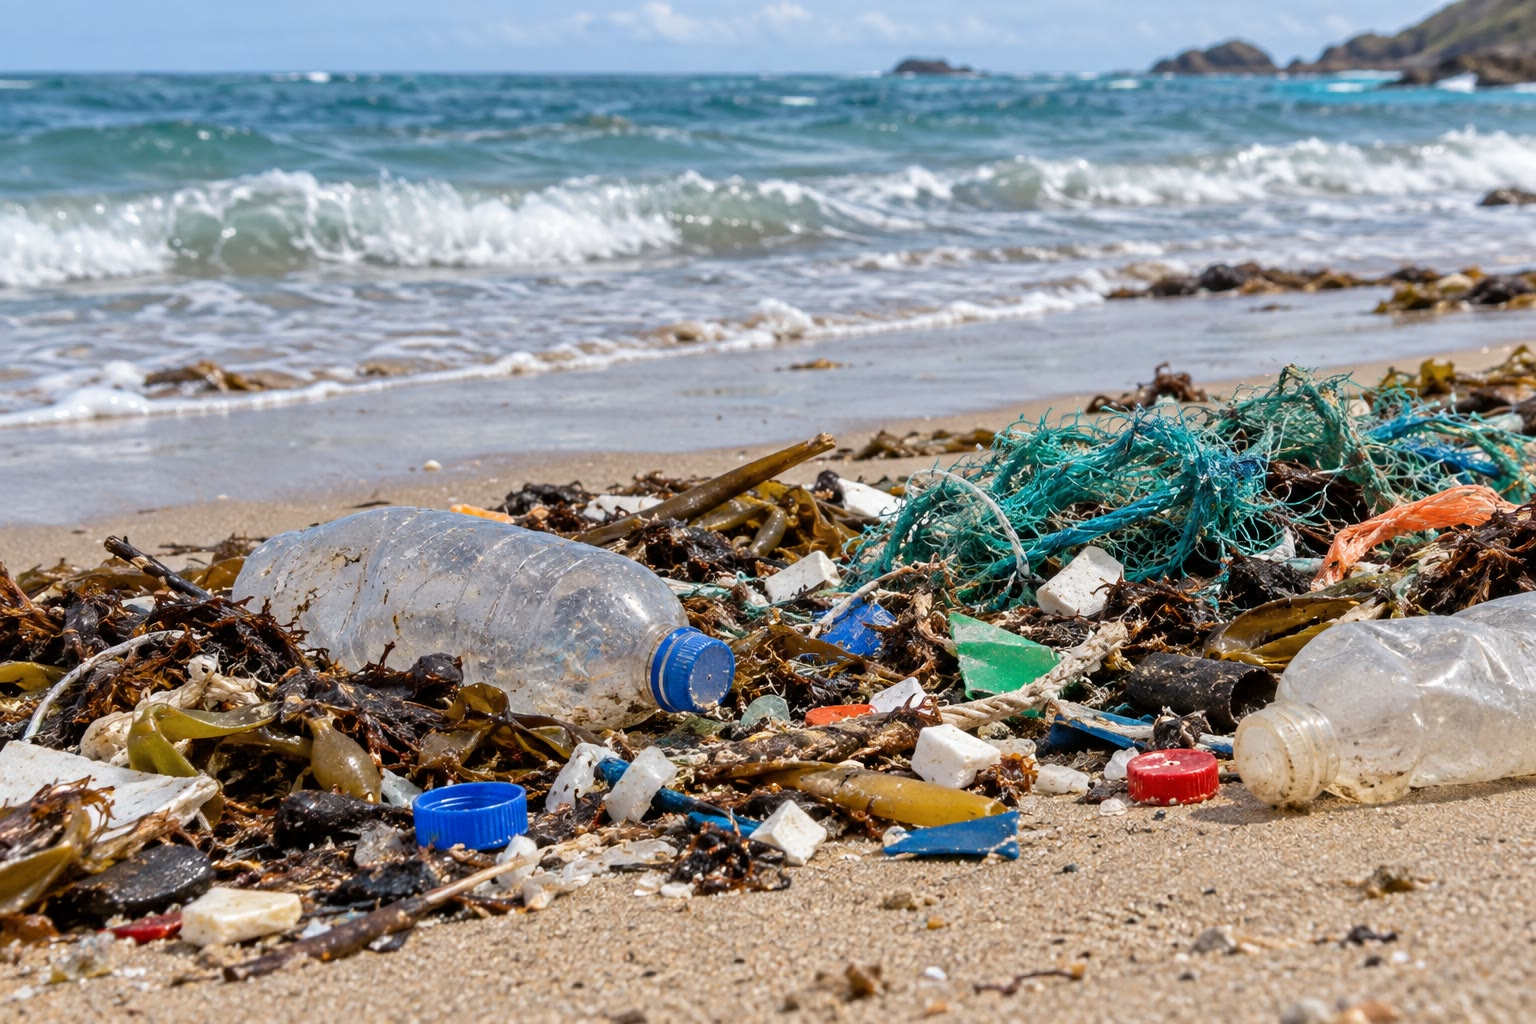
\includegraphics[width=\linewidth,height=4.6cm,keepaspectratio]{images/book1/ai/g8-beach-litter.jpg}

{\small نفايات بلاستيكية رماها الموج على شاطئ.}
\end{minipage}\hfill
\begin{minipage}[t]{0.48\linewidth}\centering
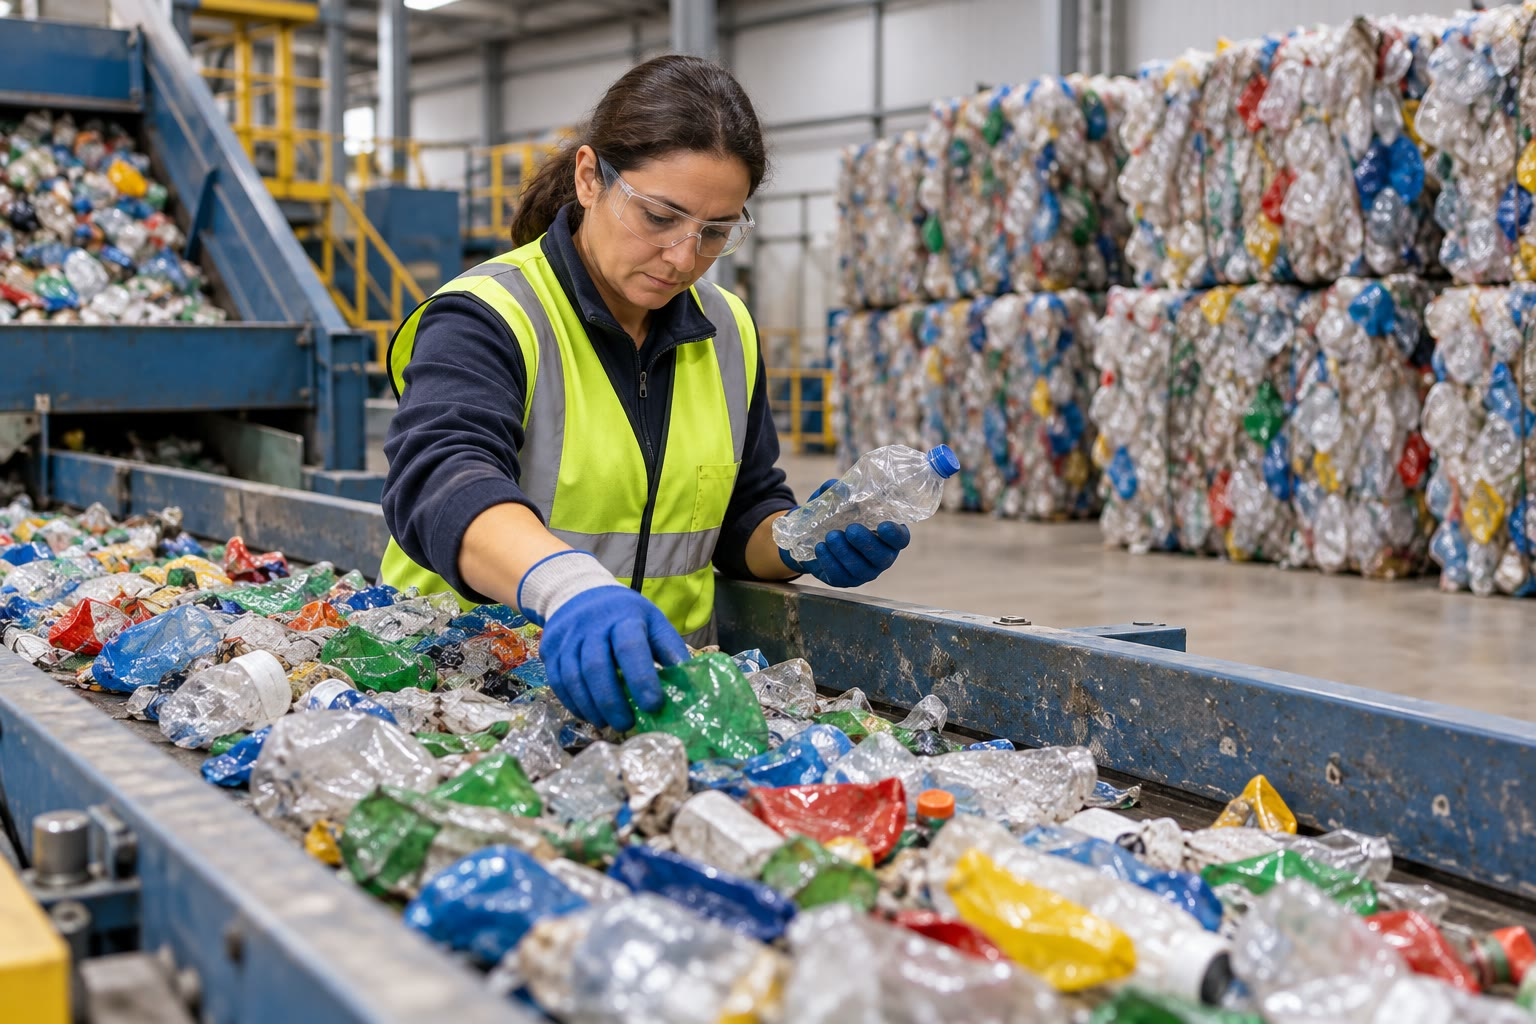
\includegraphics[width=\linewidth,height=4.6cm,keepaspectratio]{images/book1/ai/g8-sorting-line.jpg}

{\small خط فرز في مصنع لإعادة تدوير \omterm{def:g8:plastics:plastic}{البلاستيك}.}
\end{minipage}
\end{omfigure}

\begin{remark}[حرق البلاستيك]\label{rem:g8:plastics:burning}
\omterm{def:g8:plastics:plastic}{البلاستيك} يحترق، ويصنع ثنائي أكسيد الكربون حين يحترق \omterm{def:g4:what-a-fire-needs:burning}{احتراقًا} تامًا. لكنه
إذا أُحرق في نار حديقة احترق \omterm{def:g4:what-a-fire-needs:burning}{احتراقًا} غير تام وأطلق السخام وأول أكسيد
الكربون ومواد ضارة أخرى؛ \omterm{def:g8:plastics:plastic}{وبلاستيك} PVC، الذي يحوي الكلور، يطلق كلوريد
الهيدروجين، وهو غاز أكّال. ولا تُحرق نفايات \omterm{def:g8:plastics:plastic}{البلاستيك} إلا في محارق بُنيت
لتنقية أدخنتها.
\end{remark}

\section{تمارين}

\begin{exercise}[$\star$]\label{exo:g8:plastics:1}
طبيعية أم صناعية أم اصطناعية؟ القطن، والنايلون، والورق، والصوف،
والبوليستيرين، والفسكوز.
\end{exercise}

\begin{exercise}[$\star$]\label{exo:g8:plastics:2}
من أي \omterm{def:g5:raw-materials-and-recycling:raw-material}{مادة أولية} تُصنع معظم أنواع \omterm{def:g8:plastics:plastic}{البلاستيك}؟
\end{exercise}

\begin{exercise}[$\star$]\label{exo:g8:plastics:3}
أي \omterm{def:g8:plastics:plastic}{بلاستيك} رمزه 1؟ أعطِ جسمًا مصنوعًا منه.
\end{exercise}

\begin{exercise}[$\star$]\label{exo:g8:plastics:4}
ما الفرق بين \omterm{def:g8:plastics:thermoplastic}{البلاستيك الحراري} \omterm{def:g8:plastics:thermoplastic}{والبلاستيك المتصلّد بالحرارة}؟
\end{exercise}

\begin{exercise}[$\star\star$]\label{exo:g8:plastics:5}
علبة لبن تحمل الرمز 5. سمِّ بلاستيكها، وقل هل يمكن من حيث المبدأ صهرها
وإعادة قولبتها.
\end{exercise}

\begin{exercise}[$\star\star$]\label{exo:g8:plastics:6}
لماذا لا يعني مثلث الأسهم على جسم ما أن هذا الجسم سيُعاد
تدويره؟
\end{exercise}

\begin{exercise}[$\star\star$]\label{exo:g8:plastics:7}
لماذا يُصنع مقبض المقلاة كثيرًا من \omterm{def:g8:plastics:plastic}{بلاستيك} متصلّد بالحرارة لا من \omterm{def:g8:plastics:thermoplastic}{بلاستيك
حراري}؟
\end{exercise}

\begin{exercise}[$\star\star$]\label{exo:g8:plastics:8}
مستعملًا أرقام هذا الفصل لسنة 2019، ما النسبة المئوية من \omterm{def:g8:plastics:plastic}{البلاستيك} المستعمل
التي صارت نفايات في تلك السنة؟ قرّب إلى أقرب عدد صحيح.
\end{exercise}

\begin{exercise}[$\star\star$]\label{exo:g8:plastics:9}
لماذا يجب ألا يُحرق PVC أبدًا في نار حديقة؟
\end{exercise}

\begin{exercise}[$\star\star$]\label{exo:g8:plastics:10}
تستعمل مدرسة 300 قارورة كتلة كل منها \qty{25}{g} في الأسبوع، طوال 36 أسبوعًا
من السنة. ما كتلة \omterm{def:g8:plastics:plastic}{البلاستيك} هذه في سنة؟
\end{exercise}

\begin{exercise}[$\star\star\star$]\label{exo:g8:plastics:11}
البولي إيثيلين مكوّن من الكربون والهيدروجين فقط. اكتب نواتج احتراقه التام.
واشرح لماذا يضيف حرقه ثنائي أكسيد الكربون إلى \omterm{def:g4:air-a-mixture-of-gases:air}{الهواء} كما يفعل \omterm{def:g8:combustion-and-fuels:fossil}{الوقود
الأحفوري}.
\end{exercise}

\begin{exercise}[$\star\star\star$]\label{exo:g8:plastics:12}
اشرح كيف يمكن لقارورة بلاستيكية ضاعت في البحر أن تنتهي، بعد سنوات، لدائن
دقيقة داخل سمكة.
\end{exercise}

\section{مسألة: خط الفرز}

\begin{problem}[{مسألة نهاية الأسبوع --- طن من القوارير المستعملة، ورموزها،
ورقائق البلاستيك النظيفة التي تخرج من المصنع}]
\label{pb:g8:plastics:1}
يستقبل مصنع \omterm{def:g5:raw-materials-and-recycling:recycling}{لإعادة التدوير} رزمًا من قوارير المشروبات المستعملة. فرزمة نموذجية
كتلتها \qty{1}{t} (\qty{1000}{kg}) تحوي، بالكتلة: \qty{80}{\percent} من
أجسام القوارير من PET، و\qty{12}{\percent} من الأغطية (HDPE وPP)،
و\qty{5}{\percent} من الملصقات (غشاء PP) و\qty{3}{\percent} من الأوساخ
وبقايا السوائل. تفصل الآلات الأغطية والملصقات عن أجسام القوارير، وتُطحن مادة PET
رقائق، ثم تُغسل الرقائق؛ ويُفقد في الغسيل \qty{2.5}{\percent} من مادة PET.
ثم تُصهر الرقائق النظيفة وتُغزل أليافًا لسترات الصوف الاصطناعي.

\medskip
\noindent\textbf{الجزء الأول --- \omterm{def:g8:plastics:plastic}{البلاستيك}.}
\begin{enumerate}
  \item أي رمز يُطبع على أجسام القوارير؟ وعلى الأغطية؟
  \item هل هذه الأنواع من \omterm{def:g8:plastics:plastic}{البلاستيك} طبيعية أم صناعية أم اصطناعية؟
  \item هل يمكن صهر مادة PET وغزلها من جديد؟ وأي نوع من \omterm{def:g8:plastics:plastic}{البلاستيك} يجعله ذلك؟
  \item لماذا تُفصل الأغطية والملصقات عن أجسام القوارير قبل صهر
        مادة PET؟
\end{enumerate}

\medskip
\noindent\textbf{الجزء الثاني --- الرزمة.}
\begin{enumerate}[resume]
  \item ما كتلة مادة PET في الرزمة؟
  \item ما كتلة الأغطية؟ وما كتلة الملصقات؟
  \item ما كتلة الجزء الذي ليس بلاستيكًا من الرزمة؟
  \item ما النسبة المئوية \omterm{def:g8:plastics:plastic}{للبلاستيك} في الرزمة؟
\end{enumerate}

\medskip
\noindent\textbf{الجزء الثالث --- الرقائق.}
\begin{enumerate}[resume]
  \item ما كتلة مادة PET التي تُفقد في الغسيل؟
  \item تحتاج سترة من الصوف الاصطناعي إلى \qty{0.39}{kg} من ألياف PET. لماذا
        يُفضَّل صنعها من الرقائق لا من PET جديد؟
  \item يستطيع المصنع أن يحرق الأغطية والملصقات للحصول على الحرارة بدلًا من
        إعادة تدويرها. سمِّ الغاز الذي يضيفه ذلك إلى \omterm{def:g4:air-a-mixture-of-gases:air}{الهواء}.
  \item احسب كتلة رقائق PET النظيفة التي تعطيها رزمة واحدة.
\end{enumerate}
\end{problem}
